%%%%%%%%%%%%%%%%%%%%%%%%%%%%%%%%%%%%%%%%%%%%%%%%%%%%%%%%%%%%%%%
%
% Welcome to Overleaf --- just edit your LaTeX on the left,
% and we'll compile it for you on the right. If you open the
% 'Share' menu, you can invite other users to edit at the same
% time. See www.overleaf.com/learn for more info. Enjoy!
%
%%%%%%%%%%%%%%%%%%%%%%%%%%%%%%%%%%%%%%%%%%%%%%%%%%%%%%%%%%%%%%%
\documentclass{beamer}
\usepackage{tikz}
\usetheme{Copenhagen}
\usecolortheme{default}
\usepackage{subcaption}
\usepackage{wrapfig}
\usepackage{svg}

\setbeamerfont{footnote}{size=\tiny}

\newcommand{\lf}{\left[}
\newcommand{\rf}{\right]}
\newcommand{\ld}{\left{}
\newcommand{\rd}{\right}}
\newcommand{\lx}{\left(}
\newcommand{\rx}{\right)}


% \title[Seminar Geometry: Combinatorics and Algorithms: Small-dimensional linear programming and convex hulls made easy] %optional
% {Seminar Geometry: Combinatorics and Algorithms: Small-dimensional linear programming and convex hulls made easy}

\title[Seminar Geometry: Combinatorics and Algorithms FS25] %页脚
{Small-dimensional Linear Programming and Convex Hulls Made Easy}
\subtitle{Raimund Seidel}


% \subtitle{Demonstrating the Copenhagen theme}
\author[Teng Liu] % (optional)
{Teng Liu}

% \institute[VFU] % (optional)
% {
%   \inst{1}%
%   Faculty of Physics\\
%   Very Famous University
%   \and
%   \inst{2}%
%   Faculty of Chemistry\\
%   Very Famous University
% }

\date[]{April 3rd 2025}

% Use a simple TikZ graphic to show where the logo is positioned
% \logo{\begin{tikzpicture}
% \filldraw[color=red!50, fill=red!25, very thick](0,0) circle (0.5);
% \node[draw,color=white] at (0,0) {LOGO HERE};
% \end{tikzpicture}}

%End of title page configuration block
%------------------------------------------------------------
%The next block of commands puts the table of contents at the 
%beginning of each section and highlights the current section:

\AtBeginSection[]
{
  \begin{frame}
    \frametitle{Table of Contents}
    \tableofcontents[currentsection]
  \end{frame}
}
%------------------------------------------------------------
\begin{document}
\frame{\titlepage}
%---------------------------------------------------------


\begin{frame}{Background}
    Linear programming captures one of the most canonical and influential constrained optimization problems. \\~\
    
    More precisely, it asks to maximize or minimize a linear objective under linear
inequality and equality constraints.

% \begin{figure}[ht]
%     \centering
%     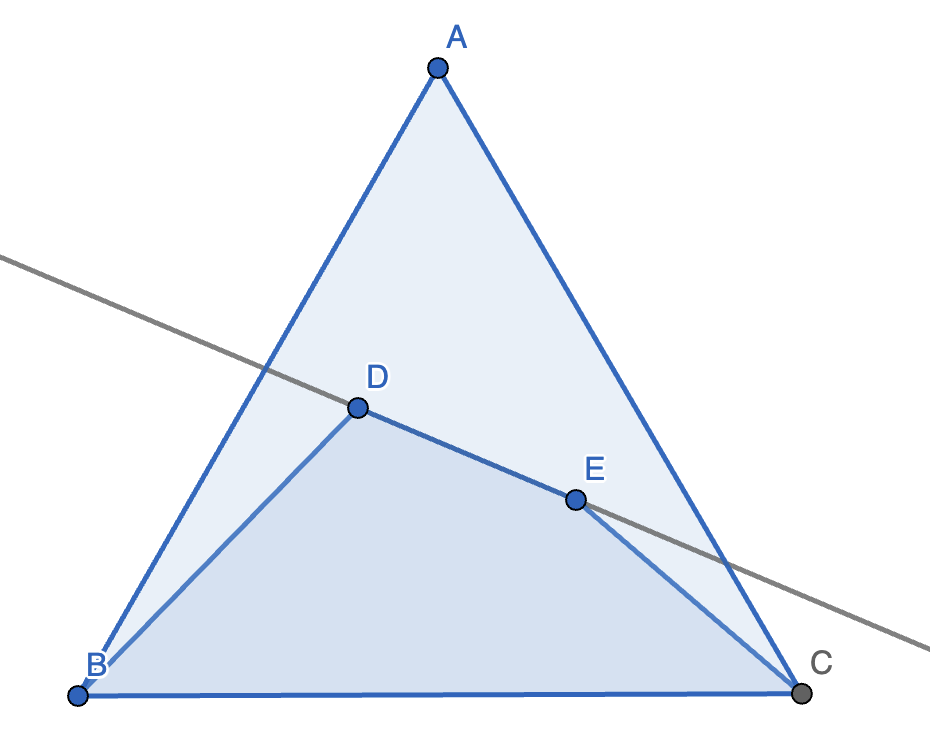
\includegraphics[width=.4\linewidth]{pre_1_1.png}
%     \caption{Five random points on a plane}
%     \label{fig11}
% \end{figure}

\begin{align*}
    \max / \min \; c^T  &x \\
   \text{subject to} \;\;\; A&x \le e \\
    B&x \ge f \\
    C&x = g
\end{align*}

% this can be interpreted as maximizing profits we get from manufacturing some products with prices respectively and a certain budgets e

\end{frame}

\begin{frame}{Background - Simplex Method}
    %% Simplex method is an impressive algorithm that solves lp in an intuitive way.
    %% 
    Fact: Optimal solution can always be achieved by some vertex. \\~\

    Each step in Simplex Method move from one vertex to the next with larger objective.
\end{frame}

\begin{frame}{Backward Analysis}
    Sometimes it's hard to determine the probability if thinking \textit{forward}, while surprisingly straightforward if thinking \textit{backward}. \\~\

    \begin{block}{Smallest Enclosing Circle}
        Given a set of points $P$ in Euclidean plane, compute the smallest circle that contains them all.
    \end{block}

    \begin{figure}[r]
        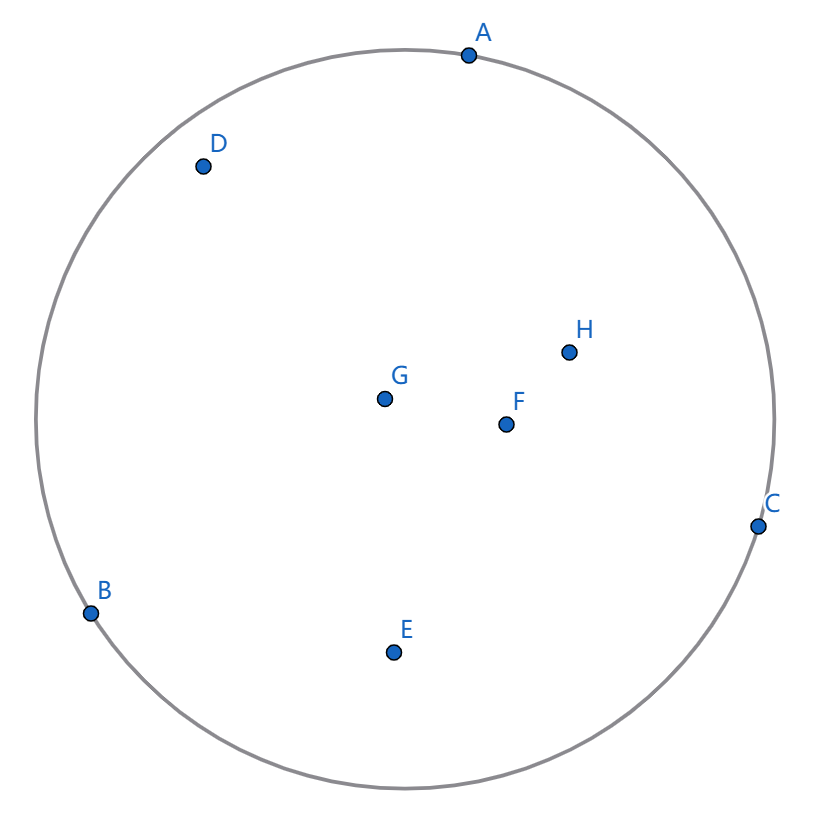
\includegraphics[width=0.4\linewidth]{pics/smallest_enclosing_circle_illustration.png}
        % \caption{}
        % \label{figsmallcircle}
    \end{figure}

    % Given first $i$ points, $\text{Pr}\lf \text{No.}(i+1) \text{ point falls in the interior of circle } C_{i+1} \rf = \;?$ \\~\

    % Given first $i+1$ points, $\text{Pr}\lf \text{No.}(i+1) \text{ point falls in the interior of circle } C_{i+1} \rf = \;?$

    % in fact, the two algorithms shares a trick in analysing some algos in common, it's called backward analysis by Seidel. the details are in depth explained in another paper where the author listed several other algorithms that backward analysis can also apply, either to give a simple proof for a previously complicated algorithm or a completely new, yet still simple proof for a new algorithm.

    % the first one is difficult to calculate because it's intrinsicly difficult. The probability differs when we have different set of first i points. So it's indeed hard to give a probability for any set of first i points, but we don't care about the probability for any specific set of first i points whatsoever: we care about only the expectation: as long as the expectation of this probability among all possible sets of first i points is bounded by some value then we are happy.

    % the second one is smarter in the sense that it doesn't depend on the set of i+1 points. whichever we choose we always have the same probability

    % here we need two pictures illustrating this:
    
\end{frame}

\begin{frame}{Backward Analysis - Smallest Enclosing Circle}
    
    Emo Welzl gave an efficient random algorithm with surprisingly simple procedure:

    \begin{figure}[h]
        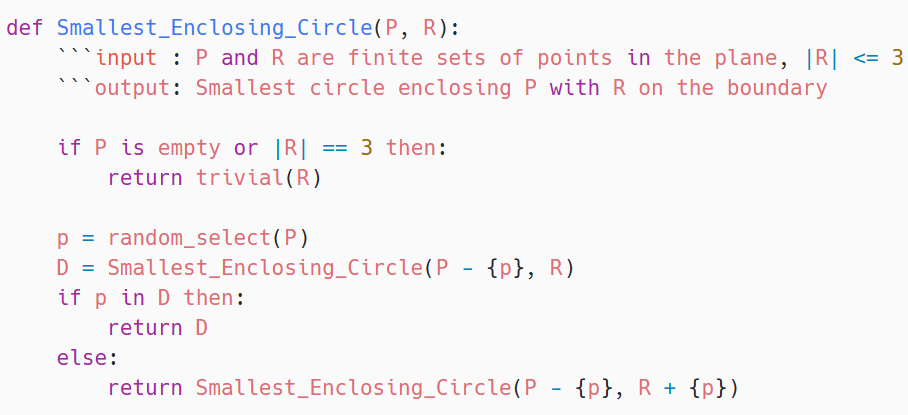
\includegraphics[width=1.0\linewidth]{pics/smallest_enclosing_circle_psudocode.png}
        % \caption{Convex hull structure: 5, 4, 3, 2.  There are 73 different structures for $n=17$.}
        % \label{figstruct}
    \end{figure}

    % Given first $i$ points, $\text{Pr}\lf \text{No.}(i+1) \text{ point falls in the interior of circle } C_{i+1} \rf = \;?$ \\~\

    % Given first $i+1$ points, $\text{Pr}\lf \text{No.}(i+1) \text{ point falls in the interior of circle } C_{i+1} \rf = \;?$

    % in fact, the two algorithms shares a trick in analysing some algos in common, it's called backward analysis by Seidel. the details are in depth explained in another paper where the author listed several other algorithms that backward analysis can also apply, either to give a simple proof for a previously complicated algorithm or a completely new, yet still simple proof for a new algorithm.

    % the first one is difficult to calculate because it's intrinsicly difficult. The probability differs when we have different set of first i points. So it's indeed hard to give a probability for any set of first i points, but we don't care about the probability for any specific set of first i points whatsoever: we care about only the expectation: as long as the expectation of this probability among all possible sets of first i points is bounded by some value then we are happy.

    % the second one is smarter in the sense that it doesn't depend on the set of i+1 points. whichever we choose we always have the same probability

    % here we need two pictures illustrating this:
    
\end{frame}

\begin{frame}{General Problem}
Can we find for a given $k$ a number $g(k)$ such that: from any set containing at least $g(k)$ points it is possible to select $k$ points forming a convex polygon\footnote{Erd\H{o}s, Szekeres: A combinatorial problem in geometry. Compositio Math. (1935)}? Such convex polygon is denoted as convex $k$-gon.

\begin{block}{Theorem}
    $g(k)$ exists for every $k \ge 3$ and $g(k) \le \binom{2k-4}{k-2} + 1$.
\end{block}

\only<1> {

\begin{figure}
\centering
    \begin{subfigure}[t]{0.3\textwidth}
        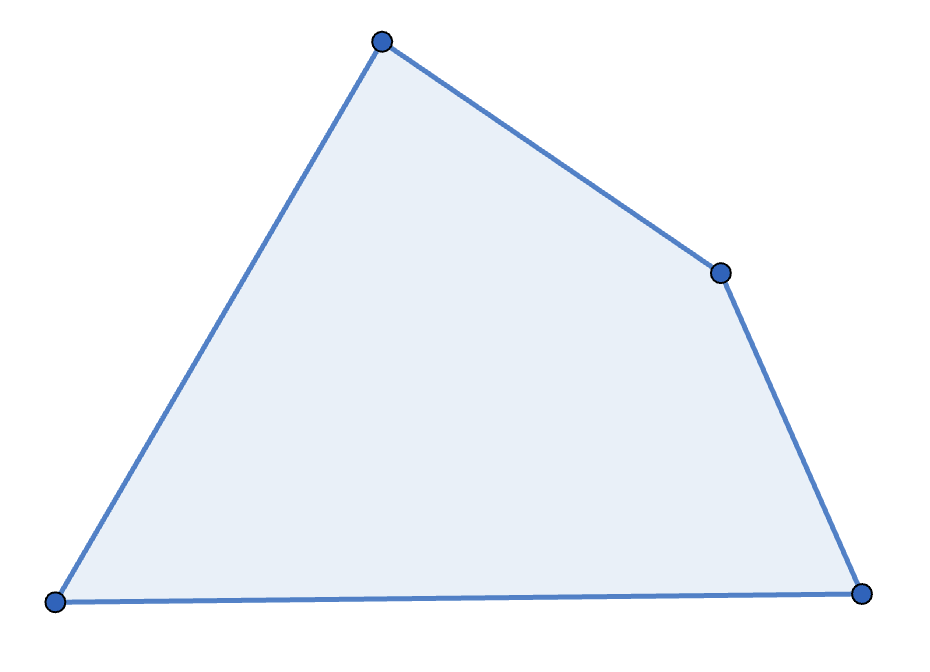
\includegraphics[width=\textwidth]{4gon.png}
        \caption{YES, convex 4-gon}
        \label{fig4gon}
    \end{subfigure}
    \begin{subfigure}[t]{0.3\textwidth}
        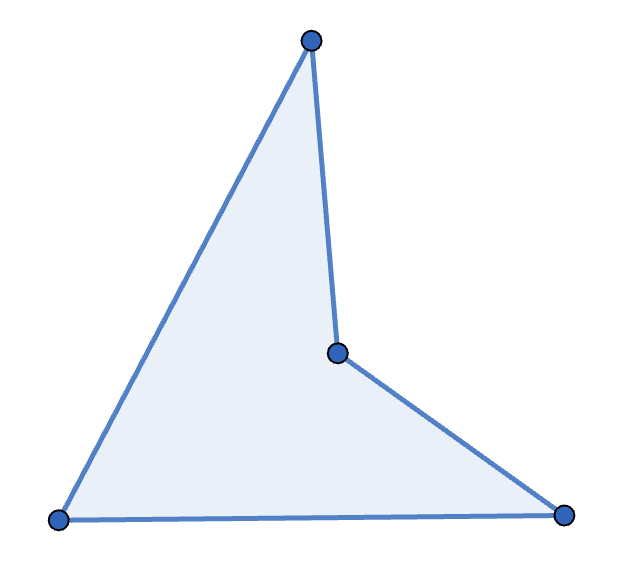
\includegraphics[width=\textwidth]{not_4gon.png}
        \caption{NO, not convex}
        \label{fignot4gon}
    \end{subfigure}
\caption{4-gons}
\label{figgons}
\end{figure}

}
% \pause 
\only<2> {
\begin{block}{Lower Bound}
    $g(k) \ge 2^{k-2} + 1$.
\end{block}

\begin{alertblock}{Conjecture}
    $g(k) = 2^{k-2} + 1$.
\end{alertblock}
}

\end{frame}

\begin{frame}{Improvements}

\begin{table}
\begin{tabular}{l | c | c }
Upper Bound & Author & Year  \\
\hline \hline
\\
$\binom{2k-4}{k-2} + 1$ & Erd\H{o}s, Szekeres & 1934 \\
\\
$\binom{2k-4}{k-2}$ & Chung, Graham\footnote{Chung, Graham: Forced convex n-gons in the plane. Discrete Comput. Geom. (1998)} & 1998 \\
\\
$2^{k + O(k ^{2/3} \log k)}$ & Suk\footnote{Suk: On the Erd\H{o}s-Szekeres convex polygon problem. J. Am. Math. Soc. (2017)} & 2017 \\
\\
$2^{k + O(\sqrt{k \log k})}$ & Holmesen et al.\footnote{Holmsen, Mojarrad, Pach, Tardos: Two extensions of the Erd\H{o}s-Szekeres problem. JEMS (2020)} & 2020
\end{tabular}
\caption{Upper Bound}
\end{table}

Asymptotically, $\Theta(2^{k+o(k)})$ is tight.

\end{frame}


\begin{frame}{Improvements}

For small $k$, some results showed the conjectured bound is tight.

\begin{itemize}
\item 
When $k=4$, we already see the proof $g(4) = 5$.
\item 
When $k=5$, Kalbfleisch et al. first gave a proof\footnote{Kalbfleisch, J.D., Kalbfleisch, J.G., Stanton, R.G.: A combinatorial problem on convex n-gons. In:
Proceedings of Louisiana Conference on Combinational Graph Theory Computing, Louisiana State University, Baton Rouge (1970)} $g(5) = 9$.
\item
When $k=6$, Szekeres and Peters\footnote{Szekeres, G., Peters, L.: Computer solution to the 17-point Erd ˝os–Szekeres problem. ANZIAM J. 48(2),
151–164 (2006)} first gave a computer-assisted proof $g(6) = 17$  using 3000 GHz Hour, while Mar\'ic\footnote{Marić, Filip. "Fast formal proof of the Erdős–Szekeres conjecture for convex polygons with at most 6 points." Journal of Automated Reasoning 62.3 (2019)} improved it to 1GHz Hour using automatic formal proof.
\end{itemize}

% \begin{wrapfig}{r}{0.5\textwidth}
% \centering
% 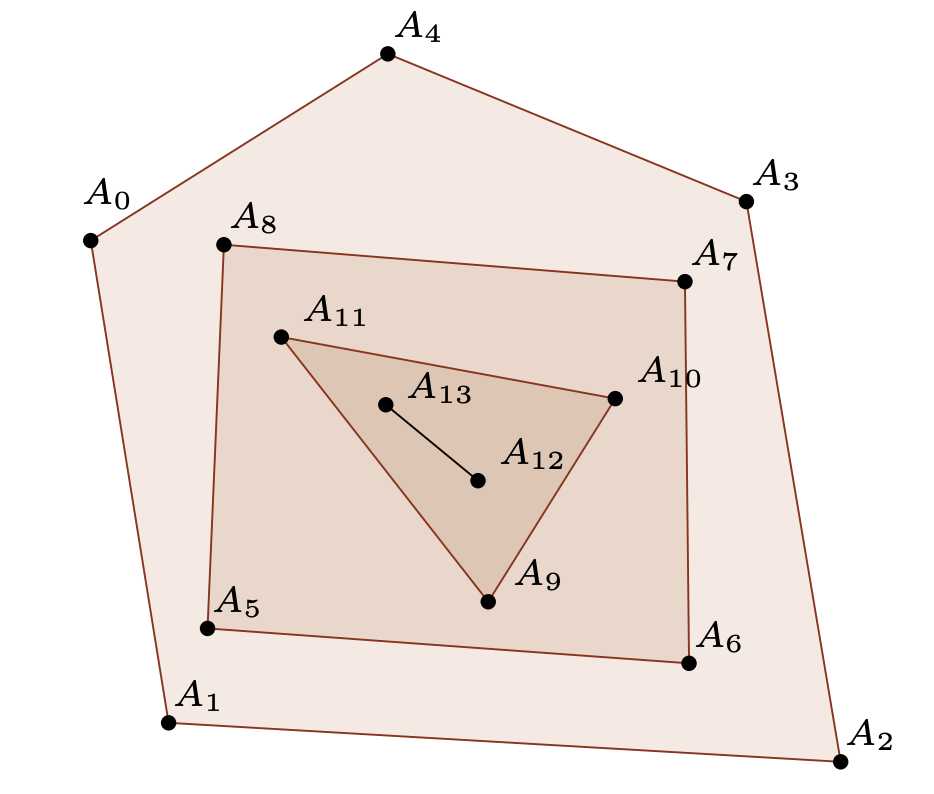
\includegraphics[width=0.2\textwidth]{convex_hull_struct.png}
% \caption{Convex hull structure}
% \end{wrapfig}

\end{frame}

\begin{frame}{Improvements}

\begin{figure}[r]
    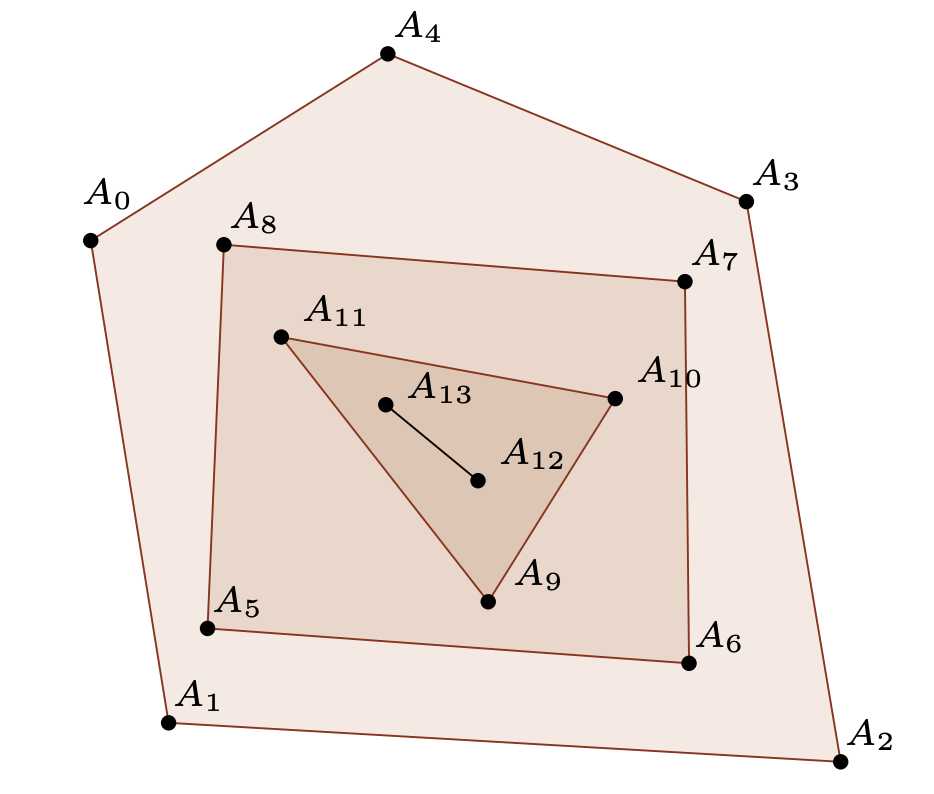
\includegraphics[width=0.7\linewidth]{convex_hull_struct.png}
    \caption{Convex hull structure: 5, 4, 3, 2.  There are 73 different structures for $n=17$.}
    \label{figstruct}
\end{figure}

\end{frame}





\begin{frame}{Holes}
Similar questions can be asked about $k$-holes, i.e. empty $k$-gons.


\begin{figure}
\centering
    \begin{subfigure}[t]{0.45\textwidth}
        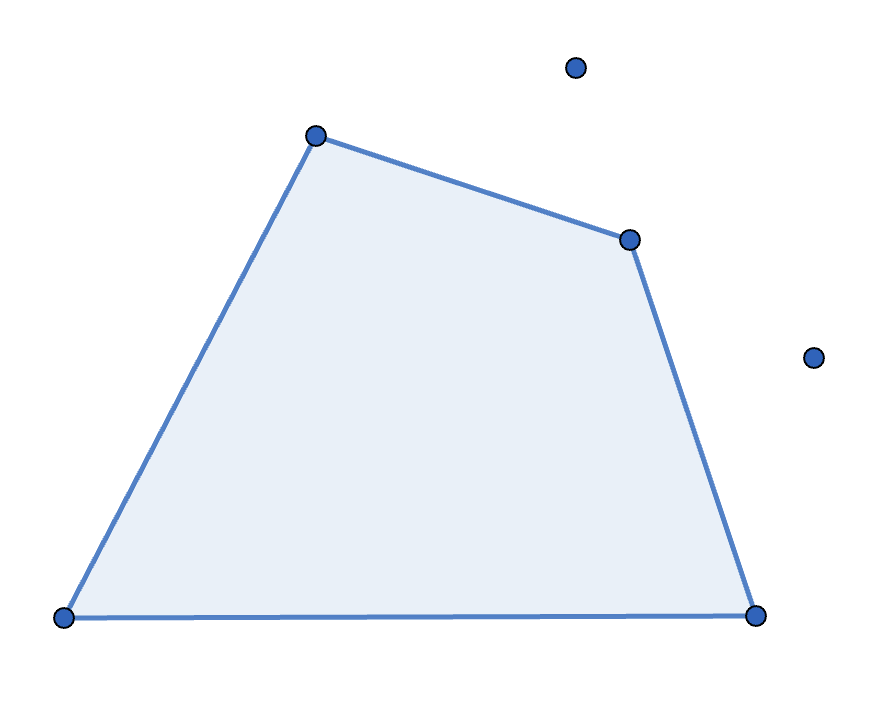
\includegraphics[width=\textwidth]{4hole.png}
        \caption{YES, convex 4-hole}
        \label{fig4hole}
    \end{subfigure}
    \begin{subfigure}[t]{0.45\textwidth}
        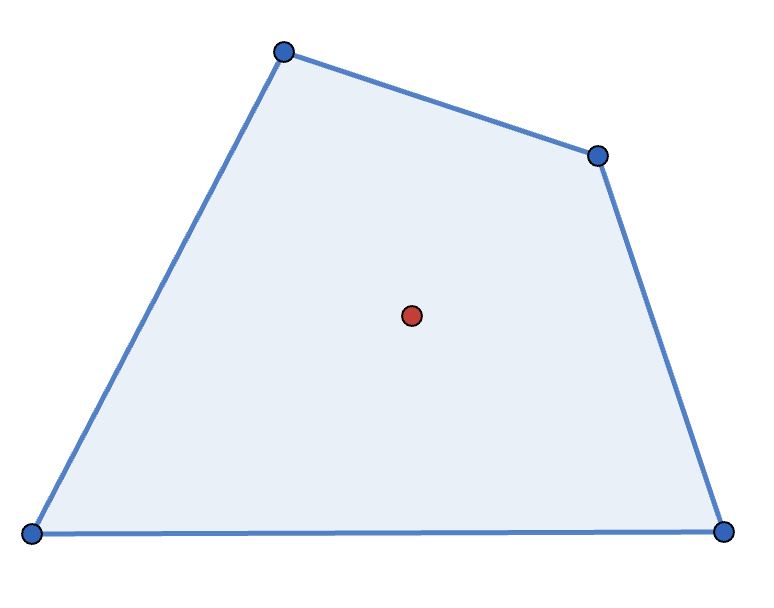
\includegraphics[width=\textwidth]{not_4hole.png}
        \caption{NO, not empty}
        \label{fignot4hole}
    \end{subfigure}
\caption{4-holes}
\label{fighole}
\end{figure}

\end{frame}

\begin{frame}{Holes}
    Similar questions can be asked about $k$-holes, i.e. empty $k$-gons. \\~\


     Can we find for a given $k$ a number $h(k)$ such that: from any set containing at least $h(k)$ points it is possible to select $k$ points forming $k$-hole?
     
\end{frame}

\begin{frame}{Holes}
    
\begin{itemize}
\item 
When $k=3$, it's trivially true that $h(3) = 3$;
\item
When $k=4$, same argument for $4$-gon can be applied to prove $h(4) = 5$.
\end{itemize}
\end{frame}


\begin{frame}{Holes}
    
\begin{itemize}
\item 
When $k=5$, Harborth et al.\footnote{Harborth, H.: Konvexe Fünfecke in ebenen Punktmengen. Elem. Math. 33, 116–118 (1978)} proved $h(5)=10$.

\end{itemize}

\begin{figure}
    \centering
    
\end{figure}


\begin{figure}
\centering
    \begin{subfigure}[t]{0.45\textwidth}
        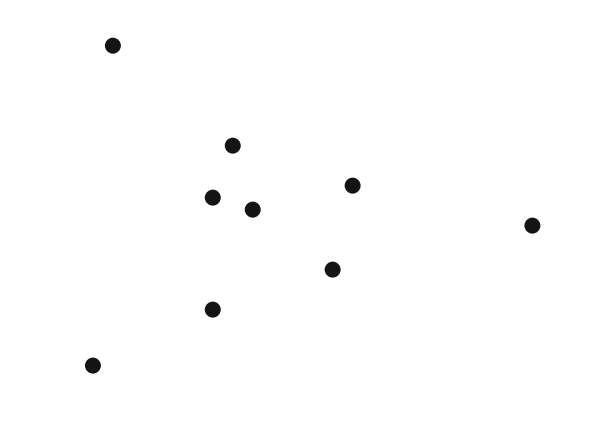
\includegraphics[width=\linewidth]{h5.png}
        \caption{9 points with no 5-hole}
        \label{fig5h}
    \end{subfigure}
    \begin{subfigure}[t]{0.5\textwidth}
        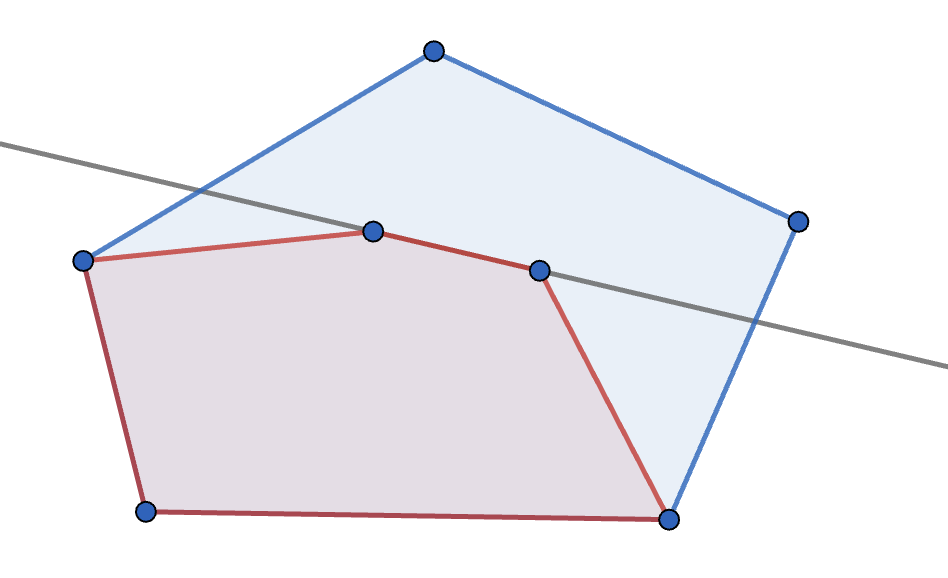
\includegraphics[width=\textwidth]{5gon-1.png}
        \caption{At least one 5-gon with only one point inside}
        \label{fig5gon1}
    \end{subfigure}
% \caption{}
\label{figk5}
\end{figure}


\end{frame}

\begin{frame}{Holes}
    
\begin{itemize}


\item 
When $k=7$, Horton\footnote{Horton, J. D.: Sets with no empty convex 7-gon. Canad. Math. Bull. 26, 482–484 (1983)} first gave a construction for  arbitrarily large $n$ points with no $7$-hole in 1983. Valtr\footnote{Valtr, P.: Convex independent sets and 7-holes in restricted planar point sets. Discrete Comput.
Geom. 7, 135–152 (1992)} gave a much simpler inductive construction  in 1992. 
\end{itemize}

\begin{figure}
\centering
        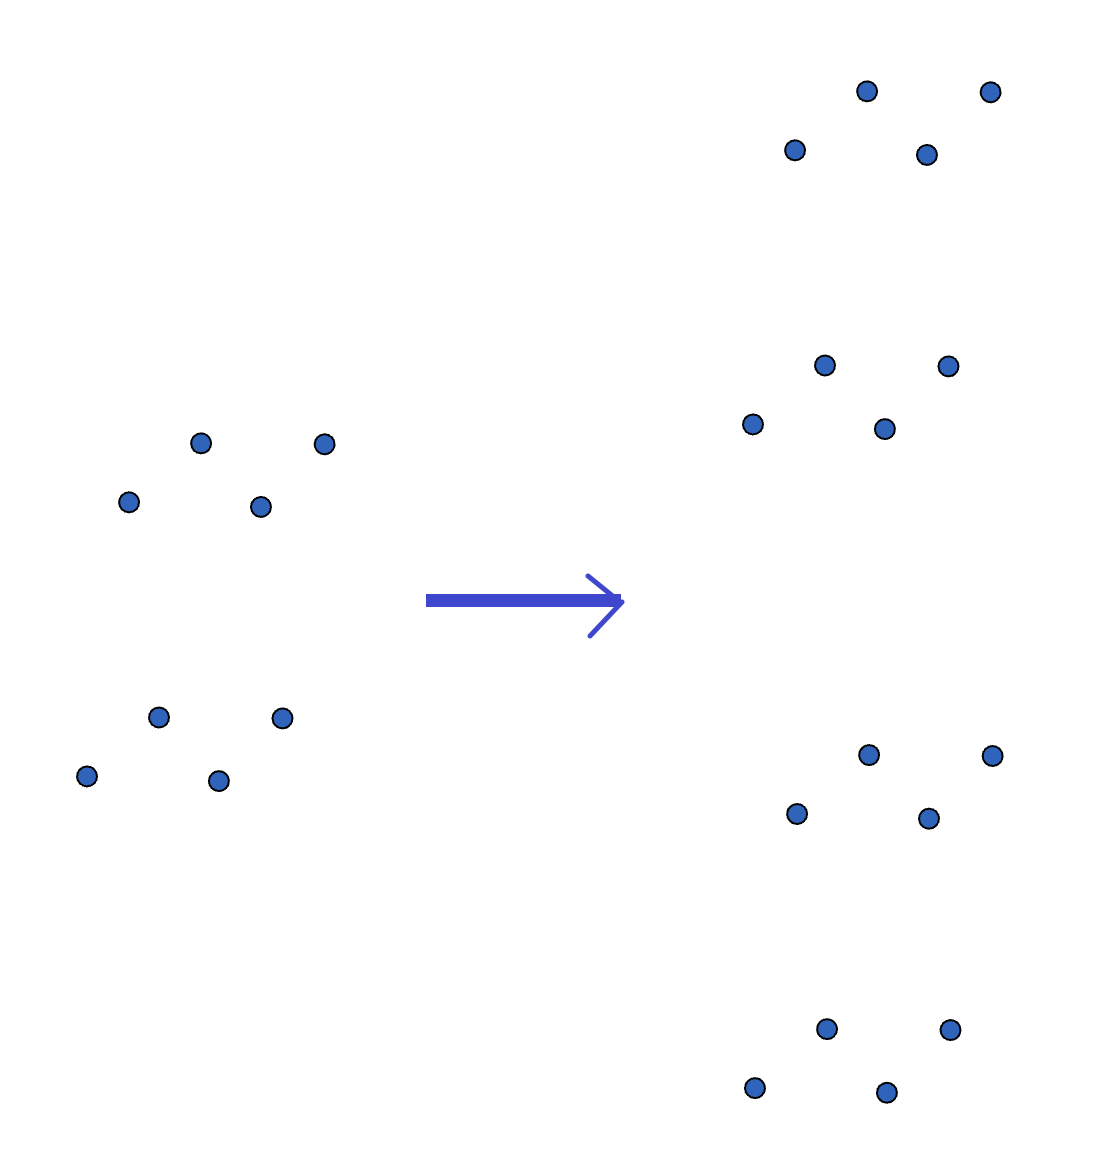
\includegraphics[width=0.5\linewidth]{7hole1.png}
        \caption{8 / 16 points with no 7-hole}

% \caption{}
\label{figh7}
\end{figure}

\end{frame}



\begin{frame}{Holes}
    
\begin{itemize}
\item 
When $k=3,4$, not quite interesting.
\item 
When $k=5$, Harborth et al. proved $h(5)=10$.
\item 

\item 
When $k=7$, Horton first gave a construction of arbitrarily large $n$ with no $7$-hole in 1983. Valtr gave a much simpler inductive construction  in 1992. 
\end{itemize}
\end{frame}


\begin{frame}{Holes}
    
\begin{itemize}
\item 
When $k=5$, Harborth et al. proved $h(5)=10$.
\item 
When $k=6$,lower bound $h(6) \ge 30$ was given by Overmars\footnote{Overmars: Finding sets of points without empty convex 6-gons. Discrete Comput. Geom.(2002)} with computer assistance; and Nicol\'as\footnote{Nicolás: The empty hexagon theorem. Discrete Comput. Geom. (2007)} proved the finiteness by showing $h(6) \le g(25)$ which was then improved by Gerken\footnote{Gerken: Empty convex hexagons in planar point sets. Discrete Comput. Geom. (2008)} to $h(6) \le g(9)$.
\item 
When $k=7$, Horton first gave a construction of arbitrarily large $n$ with no $7$-hole in 1983. Valtr gave a much simpler inductive construction  in 1992. 


\end{itemize}
\end{frame}

\begin{frame}{Variations}

What is the least number of convex $k$-gons / $k$-holes determined by any set $S$ of n points in the plane? \\~\ 

What is the least/largest number of non-convex $k$-gons / $k$-holes determined by any set $S$ of n points in the plane? \\~\ 

How to efficiently count the number of convex $k$-gons / $k$-holes?

\end{frame}

\begin{frame}{Appendix: Least Number of Convex $k$-gons / $k$-holes}

\begin{table}
\begin{tabular}{c|c}
k & Least Number \\ 
\hline \hline
4 & $\bar{cr}(n)$ \\
5 & $\Theta(n^5)$ \\ 
$\le 6$ & $\Theta(n^k)$
\end{tabular}

\caption{least number of convex $k$-gons}

\begin{tabular}{c|c}
k & Least Number \\ 
\hline \hline
3 & $n^2 - 32/7n + 22/7 \le \cdot \le 1.619n^2 + o(n^2)$ \\
4 & $n^2/2 -9/4n -o(n) \le \cdot \le 1.9397n^2 + o(n^2)$ \\ 
5 & $3n/4-o(n)\le \cdot \le 1.0207n^2 + o(n^2)$
\end{tabular}
\caption{least number of convex $k$-gons}
\end{table}
\end{frame}

\begin{frame}{Appendix: Complexity of convex $k$-gon / $k$-hole counting}

We have algorithms to with complexity $O(n^{k-2})$ and $O(kn^3)$ to count convex $k$-gons; $O(kn^3)$ and $O(kh_3(S))$ to count convex $k$-holes. \\~\ 

It's worth noting that the expected value of $h_3(S)$ is proven to be $\Theta(n^2)$ if points are uniformly chosen from a convex bounded body.
    
\end{frame}

\begin{frame}{Appendix: Ramsey Number}

Surprisingly, the finiteness of $g(k)$ can be proved with hypergraph Ramsey number. \\~\

If we color every 3-point subset $(p_i, p_j, p_k), i < j  < k$ with red if the order $(p_i, p_j, p_k)$ is clockwise order; otherwise color it with blue. \\~\

Then there exists a $k$-gon if and only if every 3-point subset of $k$ points is colored in the same color. \\~\

Thus $g(k) \le R_3(k ,k)$. And it's proven that $R_3(k, k) \le 2^{k^{k-2}\log k}$.

\end{frame}

\begin{frame}{Appendix: High Dimension Case}

Point set $S$ on $\mathbb{R}^d$ is in general  position if no $d+1$ points lie in a hyperplane; and it's convexly independent if no point lies in the convex hull of remaining points. \\~\

Similarly define $g_d(k), h_d(k)$ and we have:

\begin{itemize}
    \item 
$g_d(k) \le R_{d+2}(n, d+3)$.
    \item 
$h_d(2d+1) \le g_d(4d+1)$, which shows the existence of $h_d(k)$ if $d + 1 \le k \le 2d + 1$.
    
\end{itemize}




\end{frame}

% \end{frame}

\end{document}